%% Creator: Inkscape inkscape 0.48.0, www.inkscape.org
%% PDF/EPS/PS + LaTeX output extension by Johan Engelen, 2010
%% Accompanies image file 'single_pulse.ps' (pdf, eps, ps)
%%
%% To include the image in your LaTeX document, write
%%   \input{<filename>.pdf_tex}
%%  instead of
%%   \includegraphics{<filename>.pdf}
%% To scale the image, write
%%   \def\svgwidth{<desired width>}
%%   \input{<filename>.pdf_tex}
%%  instead of
%%   \includegraphics[width=<desired width>]{<filename>.pdf}
%%
%% Images with a different path to the parent latex file can
%% be accessed with the `import' package (which may need to be
%% installed) using
%%   \usepackage{import}
%% in the preamble, and then including the image with
%%   \import{<path to file>}{<filename>.pdf_tex}
%% Alternatively, one can specify
%%   \graphicspath{{<path to file>/}}
%% 
%% For more information, please see info/svg-inkscape on CTAN:
%%   http://tug.ctan.org/tex-archive/info/svg-inkscape

\begingroup
  \makeatletter
  \providecommand\color[2][]{%
    \errmessage{(Inkscape) Color is used for the text in Inkscape, but the package 'color.sty' is not loaded}
    \renewcommand\color[2][]{}%
  }
  \providecommand\transparent[1]{%
    \errmessage{(Inkscape) Transparency is used (non-zero) for the text in Inkscape, but the package 'transparent.sty' is not loaded}
    \renewcommand\transparent[1]{}%
  }
  \providecommand\rotatebox[2]{#2}
  \ifx\svgwidth\undefined
    \setlength{\unitlength}{354.60809303pt}
  \else
    \setlength{\unitlength}{\svgwidth}
  \fi
  \global\let\svgwidth\undefined
  \makeatother
  \begin{picture}(1,0.94591173)%
    \put(0,0){\includegraphics[width=\unitlength]{single_pulse.ps}}%
    \put(0.0,0.0518375){\makebox(0,0)[lb]{\smash{0}}}%
  
    \put(0.0,0.14){\makebox(0,0)[lb]{\smash{1}}}%
 
    \put(0.0,0.23){\makebox(0,0)[lb]{\smash{2}}}%
 
    \put(0.0,0.32){\makebox(0,0)[lb]{\smash{3}}}%
 
    \put(0.0,0.411){\makebox(0,0)[lb]{\smash{4}}}%
 
    \put(0.05,0.0){\makebox(0,0)[lb]{\smash{0}}}%
    \put(0.176,0.0){\makebox(0,0)[lb]{\smash{1}}}%
    \put(0.31,0.0){\makebox(0,0)[lb]{\smash{2}}}%
    \put(0.44,0.0){\makebox(0,0)[lb]{\smash{3}}}%
    \put(0.576,0.0){\makebox(0,0)[lb]{\smash{4}}}%
    \put(0.716,0.0){\makebox(0,0)[lb]{\smash{5}}}%
    \put(0.85,0.0){\makebox(0,0)[lb]{\smash{6}}}%
    \put(0.98,0.0){\makebox(0,0)[lb]{\smash{7}}}%
    \put(-0.03,0.22){\rotatebox{90}{\makebox(0,0)[lb]{\smash{$T$\,(эВ)}}}}%
    \put(0.48,-0.07){\makebox(0,0)[lb]{\smash{$t$,(мкс)}}}%
    \put(0.0,0.48781172){\makebox(0,0)[lb]{\smash{0}}}%
    \put(0.0,0.85){\makebox(0,0)[lb]{\smash{1}}}%
    \put(-0.03,0.6){\rotatebox{90}{\makebox(0,0)[lb]{\smash{$U$\,(у.е.)}}}}%
    %\put(0.49229724,0.93337394){\makebox(0,0)[lb]{\smash{Single pulse}}}%
    \put(0.65,0.85027601){\color[rgb]{0,0,0}\makebox(0,0)[lb]{\smash{Огибающая}}}%
    \put(0.748,0.79){\color[rgb]{0,0,0}\makebox(0,0)[lb]{\smash{накачки}}}   %  
    \put(0.76,0.41053687){\color[rgb]{0,0,0}\makebox(0,0)[lb]{\smash{Отклик}}}%
  \end{picture}%
\endgroup
